\documentclass[11pt,a4paper]{article}

\usepackage[ngerman]{babel}
\usepackage[TS1,T1]{fontenc}
\usepackage[utf8x]{inputenc}
\usepackage{theorem}
\usepackage[scaled=0.9]{helvet}
\usepackage{amsmath}
\usepackage{amssymb}
\usepackage[T1]{fontenc}
\usepackage{hyperref}
\usepackage{stmaryrd}
\usepackage{pgf,tikz}
\usepackage{relsize}
\usepackage{enumitem}
\usepackage{graphicx}
\usepackage{algpseudocode,amsmath,xifthen}
\usepackage{multicol}

\newcounter{numb}
\theoremstyle{break}
\theorembodyfont{\upshape}
   	\newtheorem{aufgabe}{Aufgabe}[numb]
\setcounter{numb}{5}
\setlength{\oddsidemargin}{0cm}
\setlength{\textwidth}{16cm}
\setlength{\textheight}{23cm}
\setlength{\topmargin}{-2cm}

\usetikzlibrary{shapes,arrows,automata,positioning,decorations.fractals}
\renewcommand\familydefault{\sfdefault}


\begin{document}

\begin{minipage}[b]{\textwidth}
\parbox[t]{5cm}{%

\includegraphics[width=4cm]{unilogo}
\hfill
}
\parbox[b]{11cm}{%
%\scshape%
Heinrich-Heine-Universit\"at D\"usseldorf\\
Institut f\"ur Informatik\\
Lehrstuhl Softwaretechnik und Programmiersprachen\\
%Professor Dr.\ M.\ Leuschel
Philipp K\"orner
}

%%date
%\hfill 1.\@ August 2017\rule{0mm}{6mm}\quad\ %% <--
\end{minipage}
\begin{center}
\bf
Funktionale Programmierung -- WS 2020 / 2021\\
Reading Guide 5: Simplicity
\end{center}

\pagestyle{empty}

\paragraph{Zeitliche Orientierung:} Diese Lerneinheit sollte bis zum 10.12.2020 abgeschlossen werden.
%\paragraph{Abgabe des Lerntagebuchs} \"uber das ILIAS bis zum 16.5.2020 mit unbegrenzt Material, Nachfrist bis zum 23.5.2020 mit zwei Seiten A4.

\section{Material} 

\begin{itemize}
\item Rich Hickey: Simple Made Easy \url{https://www.infoq.com/presentations/Simple-Made-Easy/}
\item Rich Hickey: Simplicity Matters \url{https://www.youtube.com/watch?v=rI8tNMsozo0} (22:02 -- 33:36)
\item Stuart Halloway: Simplicity Ain't Easy \url{https://www.youtube.com/watch?v=cidchWg74Y4}
\item Ben Moseley, Peter Marks: Out of the Tar Pit \url{https://github.com/papers-we-love/papers-we-love/blob/master/design/out-of-the-tar-pit.pdf} (Sektionen 1 -- 7)\footnote{Der relevante Teil des Artikels ist relativ lang, aber einfach zu lesen.}
\item The Joy of Clojure, Kapitel 14
\end{itemize}


\section{Lernziele}

Nach dem Bearbeiten dieser Lerneinheit sollten Sie in der Lage sein

\begin{itemize}
    \item die Begriffe simple, easy, hard und complex zu definieren und voneinander abzutrennen.
    \item Komplexit\"at zu erkennen.
    \item Ans\"atze zu beschreiben, mit denen man Programme verstehen kann.
    \item Ursachen von Komplexit\"at zu benennen und zu identifizieren.
    \item den Einfluss von Zustand zu beschreiben.
    \item Unterschiede in den Ans\"atzen der funktionalen und objektorientierten Programmierung bez\"uglich Komplexit\"at zu beschreiben.
    \item essentielle und nicht-essentielle Arten von Komplexit\"at zu unterscheiden und zu identifizieren.
\end{itemize}



\section{Aufgaben}

\begin{aufgabe}[Fixpunktalgorithmus]

Auf Blatt 3 haben Sie das Newton-Verfahren implementiert.
In dieser Aufgabe geht es darum, die L\"osung zu einem allgemeinen Fixpunktverfahren zu abstrahieren.
Das Newton Verfahren ist dann ein Spezialfall.
Gehen Sie dazu wie folgt vor:
    
\begin{enumerate}[label=\alph*)]
\item Schreiben Sie eine Funktion \texttt{(defn fixedpoint [F guess eps?] ...)}, das ausgehend von einem Startwert guess einen Fixpunkt von F berechnet.
    Die Genauigkeit eps? soll selber eine Funktion sein, die zwei Eingaben (den neuen Wert und den alten Wert) bekommt und true liefert, falls die beiden Eingaben hinreichend gut \"ubereinstimmen.

    Sie k\"onnen als Grundlage folgenden Code verwenden (oder Ihre eigene L\"osung):

\begin{verbatim}
(defn newton [f f']
  (fn newton-fn [x eps]
    (let [next-x (- x (/ (f x)
                         (f' x)))]
      (if (< (abs (- next-x x)) eps)
        next-x
        (newton-fn next-x eps)))))
\end{verbatim}

\item Schreiben Sie das Newton Verfahren als Instanz der Fixpunkt-Funktion.
\item Welche Aspekte der Implementierung des Newton-Verfahrens haben Sie hier abstrahiert und decomplected?
    \end{enumerate}
\end{aufgabe}

\begin{aufgabe}[Graph]
Es sollen verschiedene Funktionen auf einem Graph implementiert werden. Als Repr\"asentation des Graphen verwenden wir eine Map.

\begin{multicols}{2}[]
\begin{verbatim}
(def g {:nodes #{:a :c :b :d :e}, 
        :edges #{[:b :c] [:e :e] 
                 [:c :e] [:a :d] 
                 [:a :e] [:d :b] 
                 [:b :a]}})
\end{verbatim}

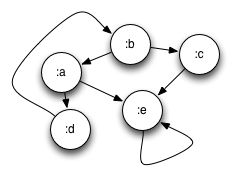
\includegraphics[width=5cm]{graph}

\end{multicols}



\begin{enumerate}[label=\alph*)]
  \item Schreiben Sie eine Funktion \texttt{(defn dom [g] ...)}, die eine Teilmenge der Knoten liefert, die eine ausgehende Kante haben.
  %(defn dom [g] (into #{} (map first (:edges g))))
  \item Schreiben Sie eine Funktion \texttt{(defn ran [g] ...)}, die eine Teilmenge der Knoten liefert, die eine eingehende Kante haben.
  %(defn ran [g] (into #{} (map second (:edges g))))
  \item Implementieren Sie eine Funktion \texttt{(defn tc [g] ...)}, die einen Graph als Parameter nimmt und einen Graph zur"uckliefert, der die transitive H\"ulle der Eingabe beschreibt. {\it Hinweis: "Uberlegen Sie, ob sie dazu die Fixpunkt-Funktion oder eine verallgemeinerte Version einer Fixpunkt-Funktion verwenden k"onnen.}
  
  \item Implementieren Sie eine Funktion \texttt{(defn trc [g] ...)}, die die transitive reflexive H\"ulle berechnet. 

  \item Schreiben Sie ein Pr\"adikat \texttt{(defn path? [g start end] ...)}, das einen truthy Wert liefert, wenn es im Graph g einen Pfad von start nach end gibt und einen falsey Wert, wenn es keinen Pfad gibt. Achten Sie darauf, dass ihr Pr"adikat auch terminiert, wenn der Graph zyklisch ist.
    \end{enumerate}
\end{aufgabe}


\section*{Fragen}
Bei Fragen wenden Sie sich bitte an Philipp K"orner (\texttt{p.koerner@hhu.de}).
\end{document}

